% AI x Epistemics Research Sprint, November 2026, Track 1.
% "A Linear Answerability Signal That the Model Does Not Act On". Every number in this deck is copied
% from the write-up (writeup/main.tex, the source of truth). Do not add numbers that are not in the write-up.
%
% Build:  ./build.sh  (or: make all)
%   main.pdf        slides only
%   main-notes.pdf  each slide followed by its speaker-notes page
\documentclass[aspectratio=169,11pt,usepdftitle=false]{beamer}

\ifdefined\withnotes
  \setbeameroption{show notes}
\else
  \setbeameroption{hide notes}
\fi

\usetheme[progressbar=frametitle,numbering=fraction,block=fill]{metropolis}
\usepackage{booktabs}
\usepackage{tikz}
\usetikzlibrary{positioning,arrows.meta,calc}
\usepackage{pgfplots}
\pgfplotsset{compat=1.18}
\usepackage{xcolor}
\usepackage{hyperref}
\setbeamerfont{note page}{size=\scriptsize}

\hypersetup{
  pdftitle={A Linear Answerability Signal That the Model Does Not Act On: Probes, Verbal Confidence and an Abstain Option in Phi-3.5-mini},
  pdfauthor={Mackenzie O'Brien, Mac Labs AI},
  pdfsubject={AI x Epistemics Research Sprint, Track 1},
  pdfkeywords={},
  pdfcreator={LaTeX Beamer},
  pdfproducer={LaTeX}
}

% ---- colors (same palette as the Lexsi deck) ----
\definecolor{stage}{RGB}{35,55,59}
\definecolor{accent}{RGB}{235,129,27}
\definecolor{auditcol}{RGB}{30,110,120}
\definecolor{stdcol}{gray}{0.50}
\definecolor{beforecol}{gray}{0.70}
\definecolor{aftercol}{RGB}{30,110,120}
\definecolor{redcol}{RGB}{170,35,45}

\newcommand{\code}[1]{\texttt{#1}}

\title{A Linear Answerability Signal\\That the Model Does Not Act On}
\subtitle{Probes, verbal confidence and an abstain option in Phi-3.5-mini}
\author{Mackenzie O'Brien, Mac Labs AI}
\institute{AI x Epistemics Research Sprint \textbullet{} Track 1: model epistemics and decision-making evals}
\date[November 2026]{November 2026}

\begin{document}

% ======================================================================
\maketitle
\note{
\begin{itemize}
\item Title follows the write-up: ``A Linear Answerability Signal That the Model Does Not Act On: Probes, Verbal Confidence and an Abstain Option in Phi-3.5-mini''.
\item Solo project for Track 1 of the AI x Epistemics Research Sprint, November 2026. All code, experiments and writing were done during the sprint.
\item Short answer up front: a linear probe on the hidden state predicts whether a question is answerable (area under the ROC curve, AUROC, 0.906). The model's stated confidence and an explicit abstain option do much worse. We do not claim the model knows it does not know.
\end{itemize}}

% ======================================================================
\begin{frame}{The question: can the model tell, and does it act on it?}
\footnotesize
\begin{columns}[T]
\begin{column}{0.50\textwidth}
\textbf{Why it matters}
\begin{itemize}
\item A model that answers every question in the same confident tone leaves its reader unable to tell which answers to trust.
\item The problem is sharpest when the evidence needed for an answer is missing.
\item This is an evaluation question: can a model's expressed confidence be checked against an internal signal and against ground truth about answerability?
\end{itemize}
\end{column}
\begin{column}{0.46\textwidth}
\textbf{What we ask}
\begin{itemize}
\item When Phi-3.5-mini-instruct reads a passage and a question the passage cannot answer, does its hidden state carry a \emph{linearly readable} trace of that fact?
\item Does anything the model \emph{says or does} (verbal confidence, token statistics, sampling agreement, an abstain option) reflect the trace?
\end{itemize}
\end{column}
\end{columns}
\begin{alertblock}{Scope}
One small model, one run, one prompt. A supervised probe shows a signal exists. It does not show the model uses it.
\end{alertblock}
\note{
\begin{itemize}
\item Motivation from the write-up's introduction: an answerer that sounds equally sure about everything is hard to trust, most of all when the passage lacks the answer.
\item Earlier work already found answerability information in hidden states (Slobodkin et al., Lavi et al., Wagner), so we do not present the existence of such a signal as new.
\item Our contribution is a controlled, fully specified measurement on a small open model, with every selection step made on validation data, and a careful account of what the behavioral comparisons do and do not show.
\end{itemize}}
\end{frame}

% ======================================================================
\begin{frame}{Setup: model, data and splits}
\scriptsize
\begin{columns}[T]
\begin{column}{0.48\textwidth}
\textbf{Model}
\begin{itemize}
\item \code{microsoft/Phi-3.5-mini-instruct}: 3.8B parameters, 32 layers, hidden size 3072
\item 8-bit quantization on one 8\,GB GPU, batch size one (the bf16 weights do not fit)
\item Greedy decoding, at most 32 new tokens; one run, seed 13
\end{itemize}
\textbf{Data}
\begin{itemize}
\item \textbf{SQuAD 2.0} (primary): 600 answerable and 600 unanswerable dev questions, split by passage 60/20/20 (720/240/240)
\item \textbf{SelfAware}: 1,000 per class, split by question 1,200/400/400
\item Pooled: \textbf{3,200 items} (1,920/640/640)
\item SQuAD test: n=240, 120 per class
\end{itemize}
\end{column}
\begin{column}{0.48\textwidth}
\textbf{Three model calls per item}
\begin{enumerate}
\item \textbf{Plain prompt}: answer, token log-probabilities and entropy, and the hidden states we probe
\item \textbf{Confidence turn}: ``How confident are you that your answer is correct?'' on 0--100
\item \textbf{Explicit abstain option}: plain prompt plus ``If the question cannot be answered, reply exactly UNANSWERABLE.''
\end{enumerate}
A hash-selected 25\% of items (807 of 3,200; 51 of the 240 SQuAD test items) also get five samples at temperature 0.7 for a consistency signal.\\[4pt]
\textbf{Scoring}: SQuAD answer correct on exact match or token-F1 $\ge 0.5$; abstention found by a rule list; no judge model.
\end{column}
\end{columns}
\note{
\begin{itemize}
\item Run: 3,200 items in 4,403 seconds. Software: torch 2.11.0, transformers 5.22.2, bitsandbytes 0.50.2, scikit-learn 1.9.1.
\item SQuAD 2.0 uses the official development set; we take 600 per class in SHA-256 hash order and split by passage so no passage appears in two splits.
\item SelfAware is subsampled to 1,000 per class from 2,338 answerable and 1,031 unanswerable questions.
\item Quantization changes hidden states slightly relative to bf16; we did not measure the effect.
\item Abstention is detected by a rule list (for example UNANSWERABLE, cannot be answered, I don't know). No model or human judge audited it.
\end{itemize}}
\end{frame}

% ======================================================================
\begin{frame}{Method: probes, baselines and what was chosen where}
\scriptsize
\begin{columns}[T]
\begin{column}{0.46\textwidth}
\textbf{Probe}
\begin{itemize}
\item Hidden state at the \emph{last prompt token}, the position that generates the first answer token, for all 33 residual positions (embedding plus 32 layers)
\item Standardized logistic regression ($C=1$), trained on the training split only; a mass-mean probe as a robustness check
\item Layer picked by \textbf{validation} AUROC
\end{itemize}
\textbf{Compared against}
\begin{itemize}
\item Verbalized confidence, mean token log-probability, negative token entropy, sampling consistency, the abstain option
\item Controls: 20 shuffled-label runs, a question-length baseline, post hoc lexical checks
\end{itemize}
\end{column}
\begin{column}{0.50\textwidth}
\scriptsize
\setlength{\tabcolsep}{3pt}
\begin{tabular}{@{}p{3.3cm}p{1.9cm}p{1.2cm}@{}}
\toprule
Choice & Made on & Reported on \\
\midrule
Probe layer (L18 for SQuAD), by AUROC & validation & test \\
Probe and confidence thresholds, by Youden's J & validation & test \\
Regularization $C=1$ and confidence cut 0.8 & fixed in config & test \\
Transfer layer, ``reported'' & source validation & target test \\
Transfer layer, ``max over layers'' & target test (optimistic) & target test \\
\bottomrule
\end{tabular}\\[6pt]
\tiny
Intervals are 95\% percentile bootstrap intervals over test items (300 resamples), ignoring clustering by passage. One seed, one split.
\end{column}
\end{columns}
\note{
\begin{itemize}
\item AUROCs are rank-based with average ranks for ties. ``The probe says unanswerable'' means a score below the threshold that maximizes Youden's J (true-positive rate minus false-positive rate) on the validation split.
\item The only quantities selected on test data are the maximum-over-layers transfer figures, which the write-up labels optimistic and does not use as headline results.
\item The shuffled-label control repeats the whole layer-wise protocol, including layer selection on validation, 20 times.
\item The length baseline is a logistic regression on question word count, question characters or prompt characters.
\end{itemize}}
\end{frame}

% ======================================================================
\begin{frame}{Result: a linear signal at middle layers}
\begin{columns}[T]
\begin{column}{0.56\textwidth}
\centering
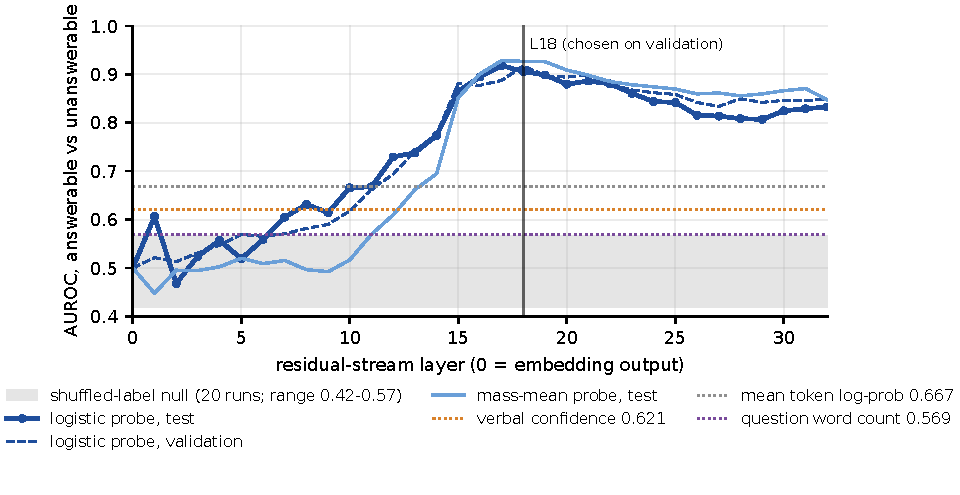
\includegraphics[width=\textwidth]{figures/fig_layers.pdf}\\
{\tiny SQuAD 2.0, n=240 per split. Shaded band: range of 20 shuffled-label runs. Vertical line: layer chosen on validation.\par}
\end{column}
\begin{column}{0.42\textwidth}
\scriptsize
\begin{itemize}
\item Test AUROC \textbf{0.906} (95\% CI 0.867--0.948) at \textbf{layer 18}, the best validation layer (validation 0.918).
\item Through layer 11 the test AUROC stays at or below 0.668; it reaches 0.865 at layer 15, peaks at 0.918 at layer 17 and falls to 0.832 at layer 32.
\item Layer 0 scores exactly 0.500, as it must when every item ends in the same token.
\item Mass-mean probe picks the same layer: 0.927 on test (validation 0.912).
\item At the validation threshold: balanced accuracy 0.821.
\item The best test layer (17) is only 0.012 above the reported value, so selection on test data does not inflate the number.
\end{itemize}
\end{column}
\end{columns}
\note{
\begin{itemize}
\item The headline: a logistic probe on the last prompt token reaches test AUROC 0.906, 95\% CI 0.867 to 0.948, at layer 18, chosen on validation AUROC (0.918).
\item Figure: test AUROC is at or below 0.668 through layer 11, rises to 0.865 at layer 15, peaks at 0.918 at layer 17 and declines to 0.832 at layer 32. Layer 0 is exactly 0.500.
\item The layer with the highest test AUROC (17) is one layer from the validation choice and 0.012 above the reported value.
\item The mass-mean (difference of class means) probe selects the same layer and reaches 0.927, so the result does not hinge on the logistic fit.
\end{itemize}}
\end{frame}

% ======================================================================
\begin{frame}{Baselines: the model's own signals do much worse}
\begin{columns}[T]
\begin{column}{0.56\textwidth}
\centering
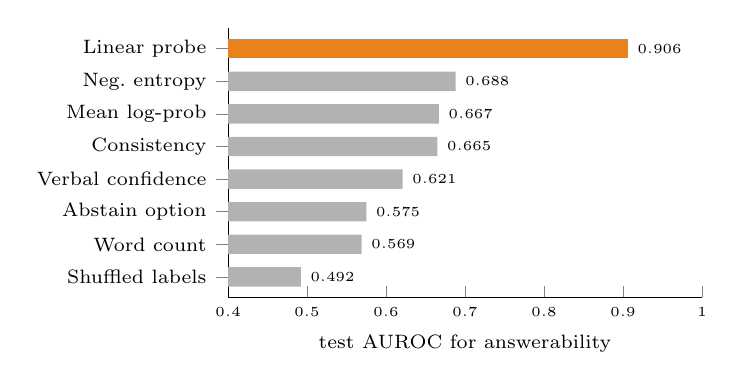
\begin{tikzpicture}
\begin{axis}[
  xbar, bar width=7pt, bar shift=0pt, width=7.6cm, height=5.0cm,
  xmin=0.4, xmax=1.0, xtick={0.4,0.5,0.6,0.7,0.8,0.9,1.0},
  xticklabel style={font=\tiny,/pgf/number format/fixed,/pgf/number format/precision=1},
  symbolic y coords={Linear probe,Neg.\ entropy,Mean log-prob,Consistency,Verbal confidence,Abstain option,Word count,Shuffled labels},
  ytick={Linear probe,Neg.\ entropy,Mean log-prob,Consistency,Verbal confidence,Abstain option,Word count,Shuffled labels}, y dir=reverse, y tick label style={font=\scriptsize},
  nodes near coords, nodes near coords style={font=\tiny,/pgf/number format/fixed,/pgf/number format/precision=3,/pgf/number format/fixed zerofill},
  axis lines*=left, enlarge y limits=0.09, clip=false, xlabel={\scriptsize test AUROC for answerability}]
\addplot[fill=beforecol,draw=none] coordinates {(0.688,Neg.\ entropy) (0.667,Mean log-prob) (0.665,Consistency) (0.621,Verbal confidence) (0.575,Abstain option) (0.569,Word count) (0.492,Shuffled labels)};
\addplot[fill=accent,draw=none] coordinates {(0.906,Linear probe)};
\end{axis}
\end{tikzpicture}\\
{\tiny SQuAD 2.0 test, n=240. Consistency covers only 51 test items. The abstain option is one hard decision, so its AUROC equals its balanced accuracy.\par}
\end{column}
\begin{column}{0.42\textwidth}
\scriptsize
\begin{itemize}
\item Verbalized confidence: \textbf{0.621} [0.558, 0.681].
\item Token-level and sampling signals: 0.665--0.688.
\item Question length: 0.569 (word count), 0.558 (characters).
\item Shuffled-label probes: mean \textbf{0.492} (SD 0.039, range 0.418--0.568, none above 0.8), so selecting a layer on 240 validation items does not by itself produce a high score.
\item Post hoc lexical checks: TF-IDF of the question 0.598, question--passage word overlap 0.600, both 0.635.
\item These baselines do not exclude other surface cues, such as how crowdworkers wrote the unanswerable questions.
\end{itemize}
\end{column}
\end{columns}
\note{
\begin{itemize}
\item Values from the write-up's signals table: probe 0.906, negative entropy 0.688, mean token log-probability 0.667 (the abstract gives 0.665--0.688 for token-level and sampling signals), verbalized confidence 0.621, abstain option 0.575, word count 0.569, shuffled labels 0.492.
\item The consistency AUROC (0.665) uses only the 51 test items that have a score, so it is not comparable with the others.
\item The bars for correctness (as opposed to answerability) are in the write-up's table; here we only show answerability.
\item Caveat: the lexical checks are post hoc; the write-up lists which numbers come from the run's analysis files and which were computed afterward.
\end{itemize}}
\end{frame}

% ======================================================================
\begin{frame}{Behavior: the model rarely abstains, with or without an option}
\scriptsize
\begin{columns}[T]
\begin{column}{0.52\textwidth}
\textbf{Plain prompt (no way to decline)}
\begin{itemize}
\item Answerable test questions answered correctly: 90.0\%
\item Abstains on \textbf{6 of 120} unanswerable items (5.0\%), and on none of the answerable ones
\item Action score 0.525 against recognition score 0.821: a recognition--action gap of \textbf{0.296} (post hoc 95\% CI 0.240--0.344)
\end{itemize}
\textbf{With the explicit UNANSWERABLE option}
\begin{itemize}
\item Abstains on \textbf{18 of 120} unanswerable items (15\%), and on none of the answerable ones
\item Precision 1.0 (18 of 18), recall 0.150 (post hoc CI 0.091--0.208), F1 0.261
\item Balanced accuracy 0.575; the gap becomes 0.246 (CI 0.189--0.292)
\end{itemize}
\end{column}
\begin{column}{0.44\textwidth}
\begin{block}{How to read this}
The option is conservative rather than inaccurate: it never refuses an answerable question, but it leaves 102 of 120 unanswerable questions answered.
\end{block}
\begin{alertblock}{Caveats}
We tried one wording of the option. The plain prompt offers no way to decline, so a low action score is expected of any model that follows the instruction.
\end{alertblock}
\end{column}
\end{columns}
\note{
\begin{itemize}
\item Definitions: the recognition score is the balanced accuracy of the probe at its validation threshold. The action score is the balanced accuracy of the model's own behavior (the mean of the share of answerable items it answers and the share of unanswerable items it abstains on). The gap is recognition minus action.
\item Under the plain prompt the model answers 90.0\% of answerable test questions correctly and abstains on 6 of 120 unanswerable ones.
\item With the explicit option the share of items with appropriate behavior moves only from 0.475 to 0.521.
\item A different wording of the option might raise recall; we tested one.
\end{itemize}}
\end{frame}

% ======================================================================
\begin{frame}{The behavioral gap: the probe flags it, the model commits anyway}
\begin{columns}[T]
\begin{column}{0.55\textwidth}
\centering
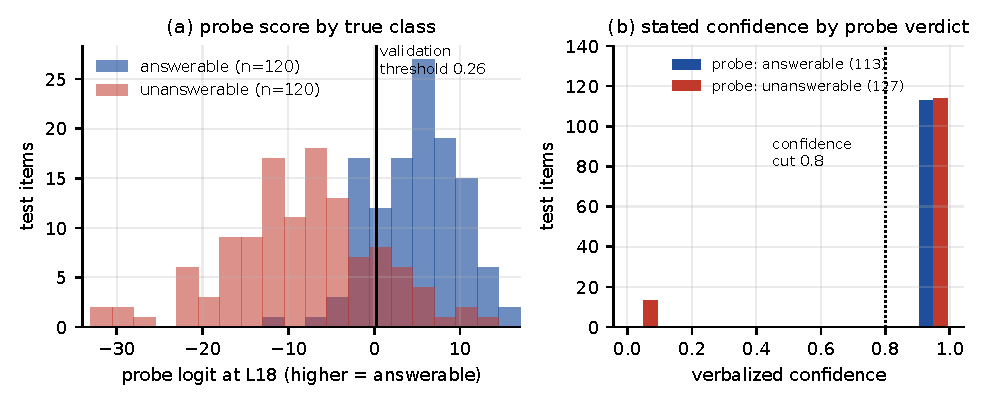
\includegraphics[width=\textwidth]{figures/fig_gap.pdf}\\
{\tiny (a) Probe logit at layer 18 by true class; the line is the validation threshold. (b) Verbalized confidence by probe verdict.\par}
\end{column}
\begin{column}{0.43\textwidth}
\tiny
\begin{itemize}
\item The probe flags \textbf{127 of 240} test items as unanswerable (102 truly so, 25 answerable).
\item Of these, 112 were answered without abstaining at confidence $\ge 0.8$: \textbf{46.7\%} of all test items (post hoc CI 41.0--52.9\%).
\item 92 of the 112 were answered wrongly: an error rate of \textbf{0.821} (CI 0.747--0.888), against 0.525 over all 240 items and 0.266 outside the gap.
\item Among the 120 unanswerable items, 87 (72.5\%) fall in the gap.
\end{itemize}
\textbf{Two limits:} the confidence condition barely filters (225 of 240 items are answered at confidence $\ge 0.8$), and the gap only shows that a probe trained on 720 labeled items recovers a distinction the model does not act on under these prompts. It does not show the model ``withholds'' anything.
\end{column}
\end{columns}
\note{
\begin{itemize}
\item Gap rate: the share of all test items where (i) the probe says unanswerable, (ii) the model did not abstain under the plain prompt, and (iii) verbalized confidence is at least 0.8.
\item Figure panel (b): all 113 items the probe calls answerable have confidence above 0.9; of the 127 it calls unanswerable, 114 do too and 13 sit near zero.
\item First limit: the confidence condition barely filters, so the gap rate is close to the share of items the probe flags and the model does not decline.
\item Second limit: the plain prompt offers no way to decline. With the explicit option the action score is 0.575 and the gap 0.246.
\end{itemize}}
\end{frame}

% ======================================================================
\begin{frame}{Flagging unanswerable items: probe, confidence and abstain option}
\small
\centering
\setlength{\tabcolsep}{6pt}
\begin{tabular}{@{}lccccc@{}}
\toprule
Rule & Recall & Precision & F1 & Coverage & False abstention \\
\midrule
\textbf{Probe, L18} & \textbf{0.850} & 0.803 & \textbf{0.826} & 0.471 & 0.185 \\
Verbal confidence $<0.95$ & 0.200 & 0.828 & 0.322 & 0.879 & 0.037 \\
Explicit abstain option & 0.150 & \textbf{1.000} & 0.261 & 0.925 & 0.000 \\
\bottomrule
\end{tabular}\\[8pt]
{\scriptsize SQuAD test, n=240 (120 unanswerable). Probe and confidence thresholds were fitted on validation labels; the abstain option used no labels. False abstention: share of correctly answered answerable items the rule would refuse.\par}
\vspace{8pt}
\begin{columns}[T]
\begin{column}{0.46\textwidth}
\footnotesize
\begin{itemize}
\item Flagging at the validation threshold keeps 47.1\% coverage and raises accuracy among answered items from 0.450 to 0.779.
\item The price: it refuses 18.5\% of correct answers.
\end{itemize}
\end{column}
\begin{column}{0.46\textwidth}
\footnotesize
\begin{itemize}
\item A cheap gate needs white-box access and labeled training data.
\item The comparison favors the probe and confidence rules, because they used validation labels and the option did not.
\end{itemize}
\end{column}
\end{columns}
\note{
\begin{itemize}
\item The probe at its validation threshold has the highest F1 and verbal confidence the next.
\item At the validation threshold the probe flags 85\% of unanswerable items at 80\% precision.
\item Practical caution from the write-up: a probe-based score presented as a certificate that an answer is supported would mislead, since 25 of its 127 flags were answerable questions and the threshold came from one benchmark.
\end{itemize}}
\end{frame}

% ======================================================================
\begin{frame}{A source confound: SelfAware looks perfect and is not evidence}
\footnotesize
\begin{columns}[T]
\begin{column}{0.50\textwidth}
\begin{itemize}
\item Probe on \textbf{SelfAware}: AUROC \textbf{0.993} [0.985, 0.998] at layer 15 (test n=400).
\item But a classifier on the \textbf{source label alone} reaches \textbf{1.000}: all 1,000 unanswerable items have source \code{SelfAware}, and none of the 1,000 answerable items does.
\item A TF-IDF classifier on the question text reaches 0.923: question style alone separates the classes.
\item Pooled probe: 0.959 [0.944, 0.972] at layer 18 (n=640), where a source-only feature gives 0.930.
\item \textbf{Transfer is weak}: SelfAware$\to$SQuAD 0.580 (layer 15); SQuAD$\to$SelfAware 0.671 (layer 18).
\end{itemize}
\end{column}
\begin{column}{0.46\textwidth}
\scriptsize
\setlength{\tabcolsep}{4pt}
\begin{tabular}{@{}lcc@{}}
\toprule
SelfAware source & Answerable & Unanswerable \\
\midrule
\code{SelfAware} & 0 & 1000 \\
\code{hotpot\_dev} & 6 & 0 \\
\code{hotpot\_train} & 64 & 0 \\
\code{squadqa\_dev} & 71 & 0 \\
\code{squadqa\_train} & 551 & 0 \\
\code{triviaqa\_dev} & 4 & 0 \\
\code{triviaqa\_train} & 304 & 0 \\
\bottomrule
\end{tabular}\\[6pt]
\footnotesize
We report SQuAD 2.0 as the primary result and SelfAware as a documented confound. Probe results on benchmarks built from mixed sources need a source audit first.
\end{column}
\end{columns}
\note{
\begin{itemize}
\item We planned to treat both datasets as probe targets. An audit changed the plan: every unanswerable SelfAware question carries the source label SelfAware.
\item The pooled probe is not at 1.000 against the source-only 0.930 because the SQuAD half shares one source across both classes.
\item Transfer maxima chosen on the target test set (0.788 at layer 19 and 0.728 at layer 10) are optimistic upper bounds and are not used as results.
\item The SQuAD to SelfAware figure is above chance but cannot separate shared answerability structure from other differences between the datasets.
\end{itemize}}
\end{frame}

% ======================================================================
\begin{frame}{What we claim, and what we do not}
\footnotesize
\begin{columns}[T]
\begin{column}{0.48\textwidth}
\textbf{The results establish}
\begin{itemize}
\item In one 3.8B model run in 8-bit, with one prompt format, a linear readout of the last prompt token at layers 15 to 19 predicts SQuAD 2.0 answerability on held-out passages (AUROC 0.906, CI 0.867--0.948, n=240).
\item That is far above a shuffled-label null (mean 0.492), a question-length baseline (0.569) and the signals the model expresses (0.621--0.688).
\end{itemize}
\end{column}
\begin{column}{0.48\textwidth}
\textbf{They do not establish}
\begin{itemize}
\item That the model represents ``not knowing''.
\item That it uses the signal, or that the signal is causal (we made no intervention).
\item That the signal transfers across datasets or generalizes to other models.
\item The SelfAware and pooled numbers are explicitly confounds; the numbers come from one seed and one split.
\end{itemize}
\end{column}
\end{columns}
\begin{alertblock}{Practical reading}
A probe is a cheap gate for white-box users (flags 85\% of unanswerable items at 80\% precision) but not a certificate that an answer is supported.
\end{alertblock}
\note{
\begin{itemize}
\item The discussion reading, that by layers 15 to 19 the prompt representation encodes whether the passage supports an answer, is a hypothesis; our experiments do not intervene on the representation.
\item We cannot separate a model limitation from an elicitation limitation: our confidence question asks about the correctness of an answer, which has no meaning for an unanswerable item, and our abstain option is a single wording.
\item Ethics section of the write-up: a headline such as ``the model knows when it does not know'' would overstate what a supervised linear probe shows; we avoid it on purpose. Possible misuse: presenting a probe score as a certificate, or using a known answerability direction to suppress abstention (reported by Lavi et al., not tested here).
\end{itemize}}
\end{frame}

% ======================================================================
\begin{frame}{Limitations}
\footnotesize
\begin{itemize}
\item \textbf{Statistical power}: the SQuAD test split has 240 items (120 per class); only 12 answerable items were answered wrongly; the consistency signal covers 51 items.
\item All comparisons reuse the same test items, with no multiple-comparison correction and no paired tests; bootstrap intervals ignore passage clustering.
\item \textbf{Measurement}: no judge audited the rule-based abstention detector; SelfAware answers are scored by string containment, which understates accuracy.
\item The probe sees only the plain prompt, while the abstain-option pass uses a different prompt, so the two are not evaluated on identical inputs.
\item Prompts were truncated at 1,024 tokens (not logged how many); 8-bit quantization may shift hidden states.
\item SQuAD's unanswerable questions were written adversarially, so surface artifacts beyond those tested may exist.
\item The abstain-option analysis code was added after the run, and its numbers were recomputed from the run's saved responses.
\end{itemize}
\note{
\begin{itemize}
\item These are the write-up's Discussion and Limitations, nearly verbatim in substance.
\item Appendix B of the write-up lists which numbers come from the run's analysis files and which we computed afterward (the post hoc bootstrap intervals, the lexical baselines and the abstain-option figures).
\item A 400-item development run gave a lower SQuAD probe AUROC (0.821 at layer 19); the write-up attributes this to the small test split (41 SQuAD items), without a further test.
\end{itemize}}
\end{frame}

% ======================================================================
\begin{frame}{What's next}
\normalsize
\textbf{Most informative next steps}
\begin{itemize}
\item An \textbf{interventional test}: add or ablate the probe direction and measure abstention, in the manner of Lavi et al.
\item A prompted answerability question and a P(True) baseline.
\item Several abstain-option wordings.
\item Multiple seeds and splits, and a second model.
\item An unconfounded inherent-unanswerability dataset in which source does not alias the label.
\end{itemize}
\note{
\begin{itemize}
\item These are the write-up's stated future work. The interventional test is the one that would turn a readable signal into a claim about use.
\item Multiple seeds and splits would also give the variance that one run cannot.
\end{itemize}}
\end{frame}

% ======================================================================
\begin{frame}{Links and references}
\small
\begin{itemize}
\item \textbf{Code (GitHub):} \url{https://github.com/mso-docs/Apart-Epistemics}
\item \textbf{Dataset (Hugging Face):} \url{https://huggingface.co/datasets/mackenzietechdocs/apart-epistemics-phi35-abstention}
\item \textbf{Landing page:} \url{https://mso-docs.github.io/Apart-Epistemics/}
\item \textbf{Data:} SQuAD 2.0 and SelfAware are public (CC BY-SA 4.0).
\end{itemize}
\vspace{4pt}
\scriptsize
\textbf{Key references} (arXiv IDs as listed in the write-up):
Phi-3 technical report (2404.14219); SQuAD 2.0, Rajpurkar et al.\ (1806.03822); SelfAware, Yin et al.\ (2305.18153); geometry of truth probes, Marks and Tegmark (2310.06824); control tasks for probes, Hewitt and Liang (1909.03368); curious case of hallucinatory (un)answerability, Slobodkin et al.\ (2310.11877); linear directions for (un)answerability, Lavi et al.\ (2509.22449).\\[4pt]
Author: Mackenzie O'Brien, Mac Labs AI (sole author). Research conducted at the AI x Epistemics Research Sprint, November 2026.
\note{
\begin{itemize}
\item Code, dataset and the landing page are linked here. The dataset holds the processed items and per-item model outputs for run 20261114T041458Z-full--apart.
\item Every figure and table in the write-up can be regenerated from the run's JSON files with the scripts in writeup/scripts.
\end{itemize}}
\end{frame}

\end{document}
